

\subsection{Subsystem 1 RC controller}
We've decided to use a double joystick RC controller for the time being. We have to spend the extra money to buy a remote controller but the benefit would be that the submarine will be easier to pilot. The other option was just using keyboard inputs from a laptop.

\begin{figure}[h!]
	\centering
 	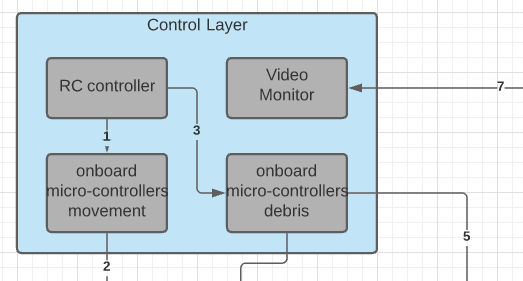
\includegraphics[width=0.60\textwidth]{images/subsystem_control}
 \caption{Example subsystem description diagram}
\end{figure}

\subsubsection{Assumptions}
We made the assumption that easier piloting will lead to higher points. We also assumed that an RC controller is going to be easier to use than keyboard inputs from a laptop.

\subsubsection{Responsibilities}
The responsibilities of the RC controller is to send the electrical signals to the laptop which will then be translated by ArduPilot into actionable instructions on the part of the micro-controllers. 

\subsubsection{Subsystem Interfaces}
Each of the inputs and outputs for the subsystem are defined here. Create a table with an entry for each labelled interface that connects to this subsystem. For each entry, describe any incoming and outgoing data elements will pass through this interface.

\begin {table}[H]
\caption {Subsystem interfaces} 
\begin{center}
    \begin{tabular}{ | p{1cm} | p{6cm} | p{3cm} | p{3cm} |}
    \hline
    ID & Description & Inputs & Outputs \\ \hline
    \#01 & USB interface through tether & \pbox{3cm}{joystick forward backward \\ joystick left-right} & \pbox{3cm}{ArduPilot library calls}  \\ \hline
    \#02 & USB interface & \pbox{3cm}{button clasp} & \pbox{3cm}{micro-controller signal}  \\ \hline
    \end{tabular}
\end{center}
\end{table}

\subsection{Subsystem 2 onboard micro-controllers movement}
\subsubsection{Assumptions}
We've made the assumption that all movement can be controlled by turning power on/off to the thrusters. 

\subsubsection{Responsibilities}
The responsibility is for the micro-controller to give power and/or cut power to the thrusters depending on how we want the submarine to move. The signals for which action the microcontrollers will take will be given via translated library calls from ArduPilot.

\subsubsection{Subsystem Interfaces}

\begin {table}[H]
\caption {Subsystem interfaces} 
\begin{center}
	\begin{tabular}{ | p{1cm} | p{6cm} | p{3cm} | p{3cm} |}
		\hline
		ID & Description & Inputs & Outputs \\ \hline
		\# & USB interface through tether & \pbox{3cm}{USB input} & \pbox{3cm}{Arduino pin signals}  \\ \hline
	\end{tabular}
\end{center}
\end{table}

\subsection{Subsystem 3 onboard micro-controllers debris}
\subsubsection{Assumptions}
we've made the assumption that we will not be able to figure out how to get the arm to clasp without some sort of electrical power solution.

\subsubsection{Responsibilities}
The responsibility of this subsystem is to force the clamp to close when we have the target in sight, and to launch the catapult debris system when it is loaded.

\subsubsection{Subsystem Interfaces}

\begin {table}[H]
\caption {Subsystem interfaces} 
\begin{center}
	\begin{tabular}{ | p{1cm} | p{6cm} | p{3cm} | p{3cm} |}
		\hline
		ID & Description & Inputs & Outputs \\ \hline
		\# & USB interface through tether & \pbox{3cm}{USB input} & \pbox{3cm}{Arduino pin signals}  \\ \hline
	\end{tabular}
\end{center}
\end{table}

\subsection{Subsystem 4 video monitor}
\subsubsection{Assumptions}
we've made the assumption that it will be impossible to pilot the submarine by looking into the water at an angle due to the light reflectivity.

\subsubsection{Responsibilities}
The responsibility of this subsystem is to display the video information being displayed to it from the camera system.

\subsubsection{Subsystem Interfaces}

\begin {table}[H]
\caption {Subsystem interfaces} 
\begin{center}
	\begin{tabular}{ | p{1cm} | p{6cm} | p{3cm} | p{3cm} |}
		\hline
		ID & Description & Inputs & Outputs \\ \hline
		\# & USB interface through tether & \pbox{3cm}{USB input} & \pbox{3cm}{video image}  \\ \hline
	\end{tabular}
\end{center}
\end{table}
